\documentclass[12pt]{article}
\usepackage{fullpage,amsfonts,amsmath,mathpazo,graphicx,verbatim,parskip,color,mdframed}
\usepackage[left=2cm,top=2cm,right=2cm,bottom=2cm,head=2cm,foot=1cm]{geometry}
\usepackage{notes}

\usepackage{notes}
\newcommand{\solution}{\textbf{Solution: }}
\renewcommand{\P}{\Pr}
\newcommand{\x}{\vec x}
\newcommand{\w}{\vec w}

\title{Machine Learning}

\begin{document}

\maketitle

\begin{itemize}
\item $n$ sample points $x_i \in \R^d$, $i = 1, \ldots, n$
\item $d = 2$ where not stated.
\end{itemize}

\section*{Classification}

A \textbf{decision boundary} is a curve separating the plane (sample space)
into two regions.

Some classifiers involve a \textbf{decision function} $f$, in which case
$f(\x) = 0$ describes the decision boundary.

A \textbf{linear classifier} uses a linear decision function
$f(x) = \w \cdot \x + \alpha$. This is scalar-valued: it's a plane over
the plane (sample space). Its intersection defines a linear decision boundary.

In $d$-dimensions the decision boundary is a hyperplane
($(d-1)$-dimensional). This still separates the sample space into two regions.

\textbf{Example:} $f(x) = \cvec{1}{1} \cdot \cvec{x_1}{x_2} + 4$
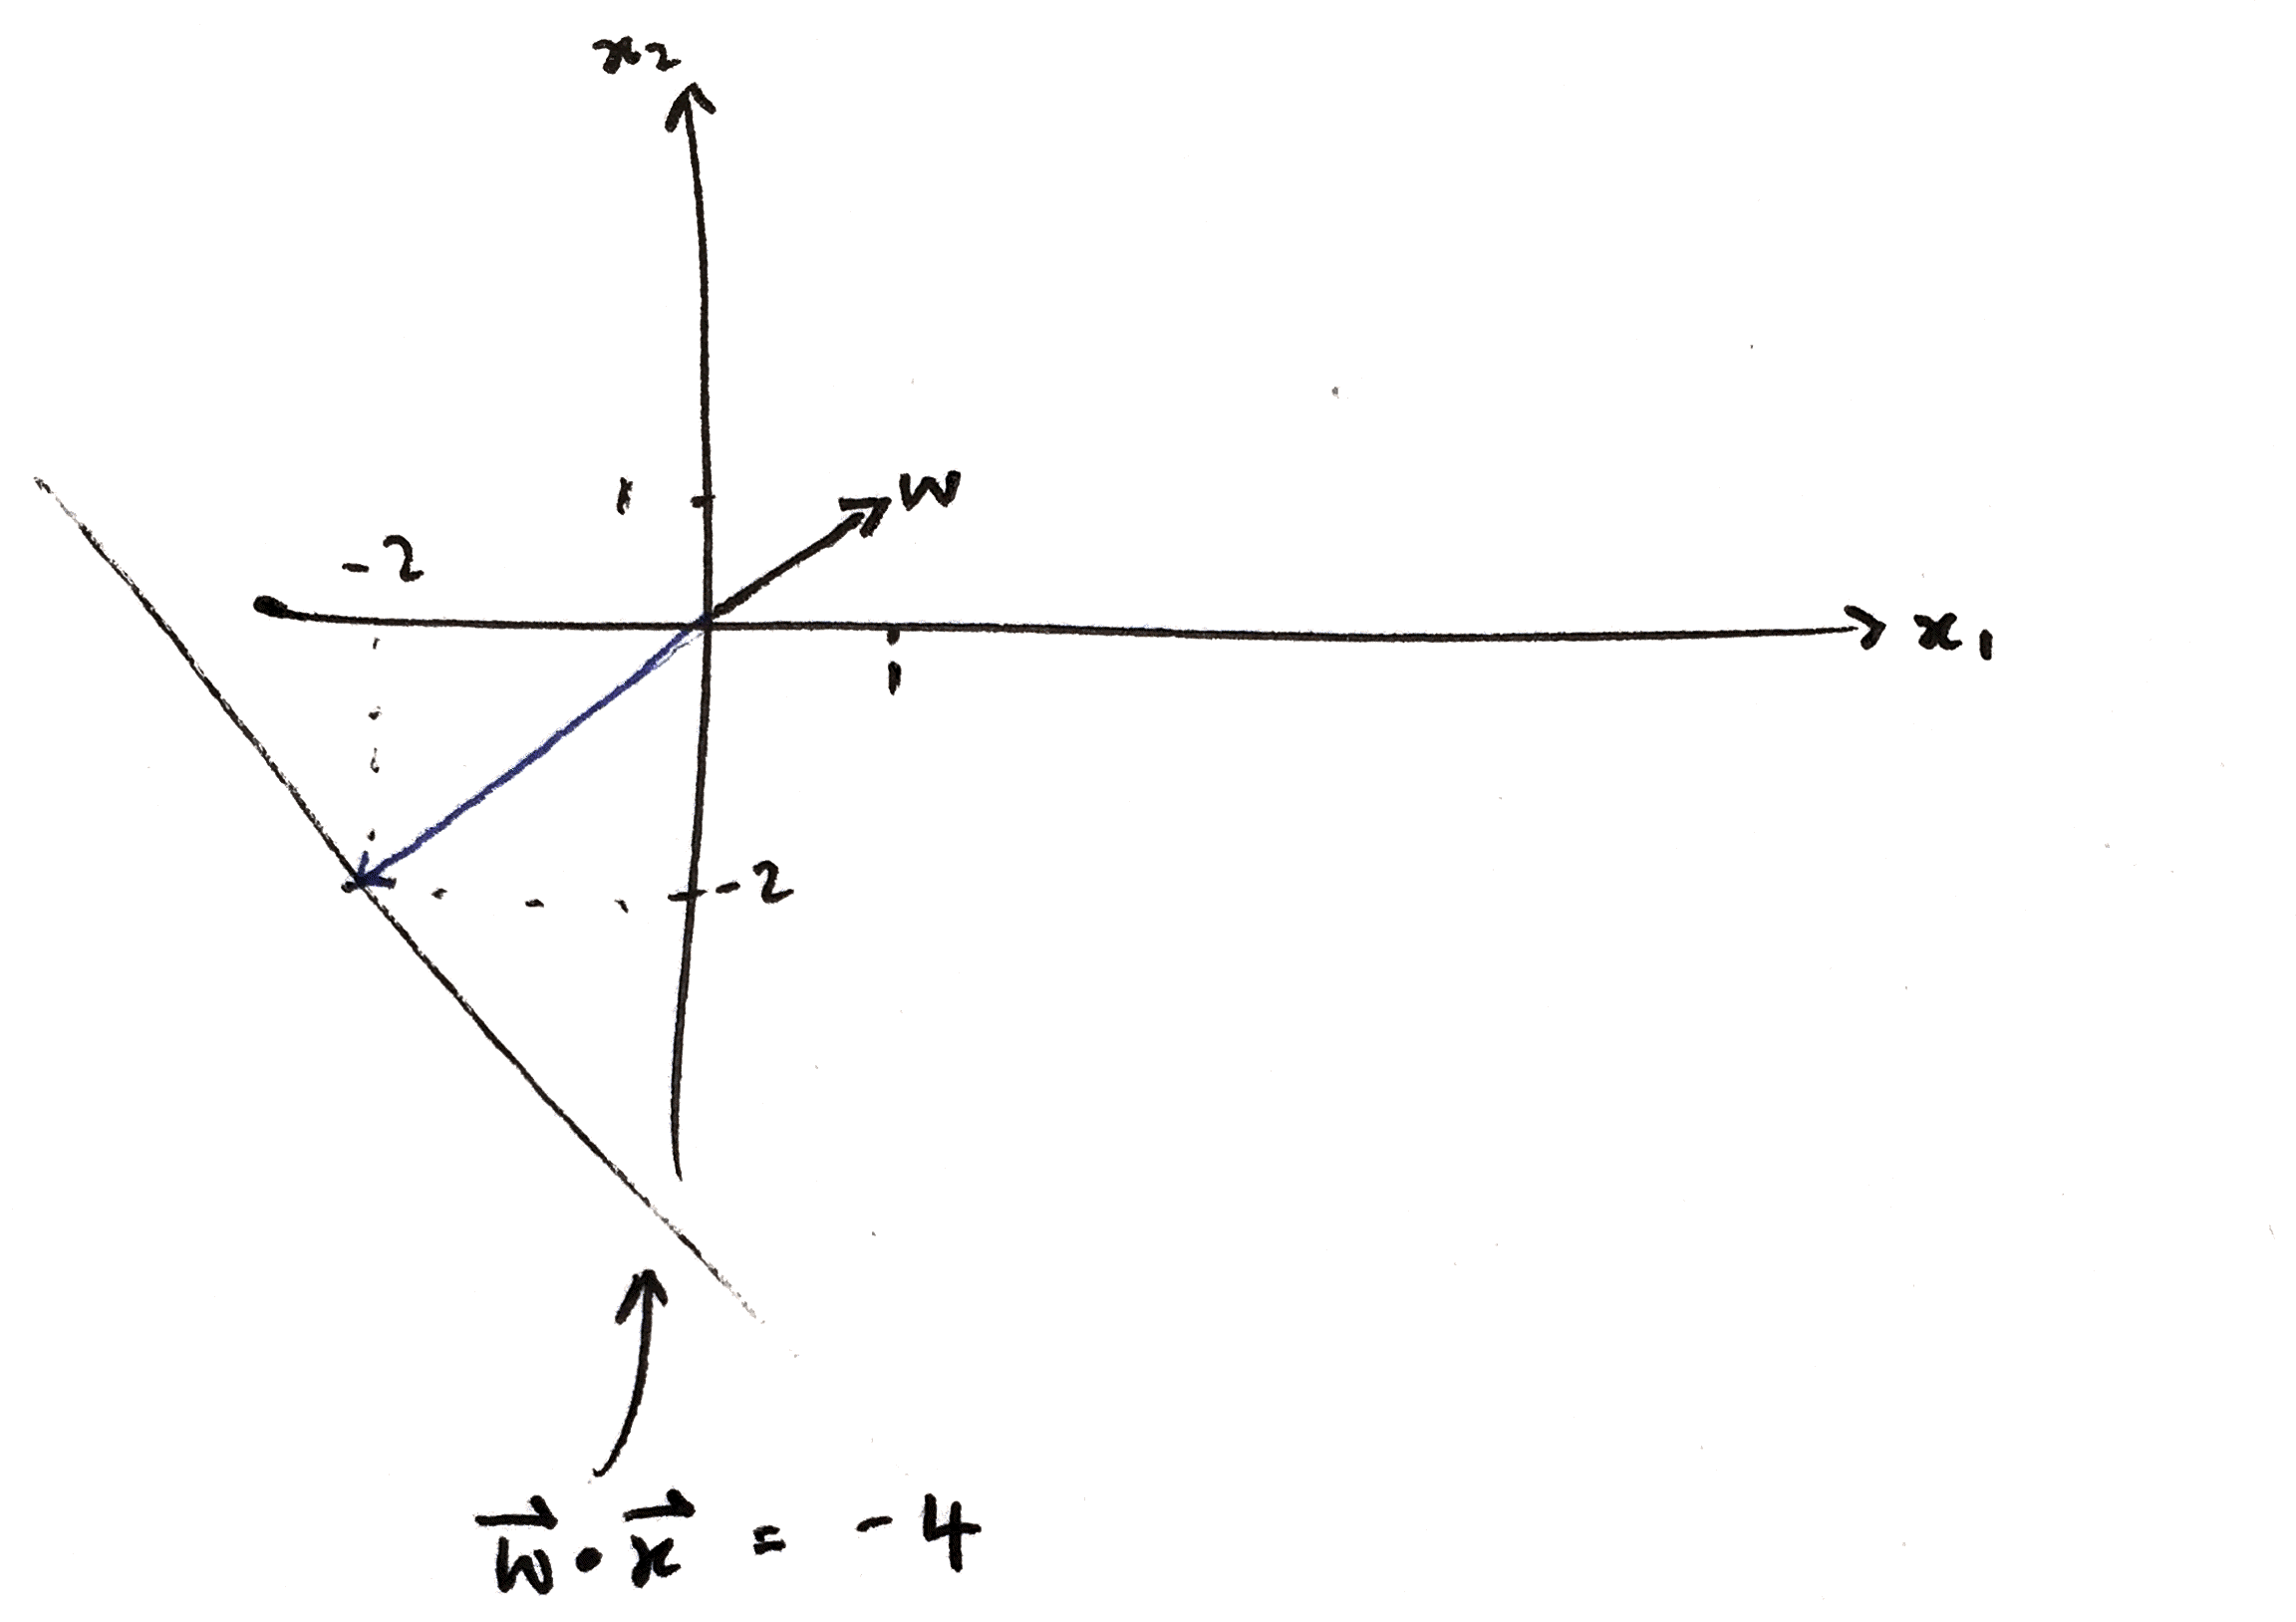
\includegraphics[width=200pt]{img/machine-learning-linear-decision-boundary.png}
\begin{itemize}
\item A plane sloping up at 45° in the north-east direction.
\item Each input feature has equal influence on the classification.
\item Decision boundary is line $x_1 + x_2 = -4$.
\item $\w$ is normal to the decision boundary since $\w \cdot (\x_1 - \x_2) = -4 - (-4) = 0$.
\item If one feature has a very high weight then $\w$ points close to that
  axis and the decision boundary is almost perpendicular to that axis (other
  features almost don't matter).
\end{itemize}

I'm still not fully comfortable with the role of $\w \cdot \x$ and the
distance of lines to the hyperplane / origin, etc:
\begin{mdframed}
  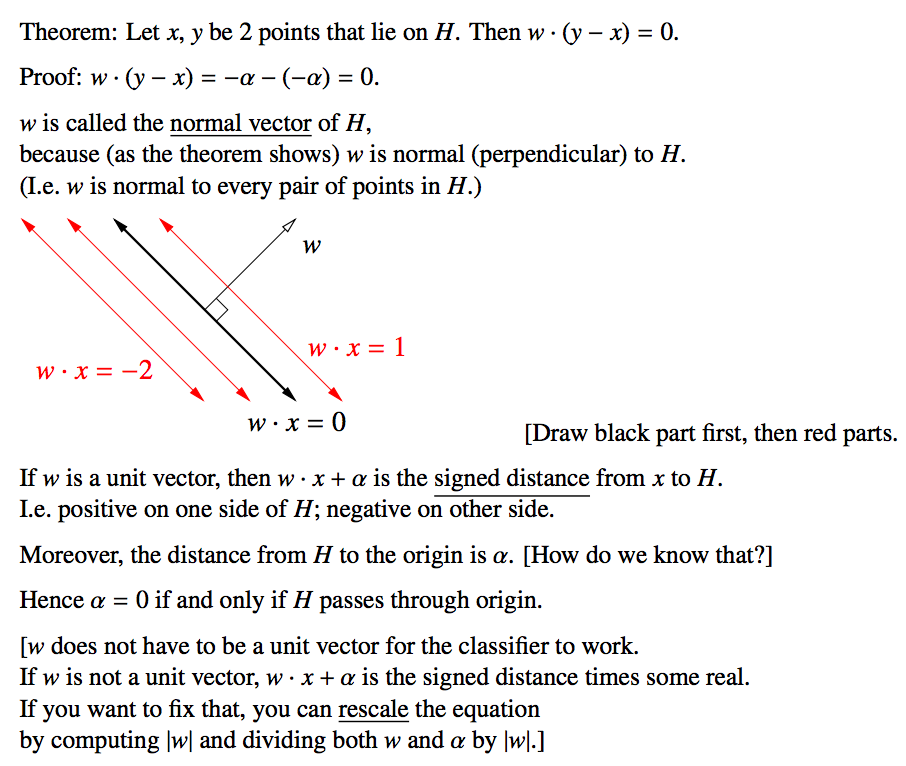
\includegraphics[width=300pt]{img/machine-learning-linear-decision-boundary-2.png}
\end{mdframed}
Examples of linear classifiers:
\begin{description}
\item[Centroid method] Decision boundary perpendicular to and bisects line
  connecting means of labeled training points.
\item[Perceptron]
\item[LDA] Fit Gaussians to each class, same covariance across classes.
\end{description}

\subsection*{Perceptron}

Labels $y_i \in \{-1, 1\}$. Assume $\alpha=0$ for now (decision boundary through origin).

\textbf{Goal}: find line separating points (separating hyperplane). I.e. Find $\w$ such that
\begin{align*}
  \begin{cases}
    \x_i \cdot \w \leq 0, &y_i = -1 \\
    \x_i \cdot \w \geq 0, &y_i = +1
  \end{cases}
\end{align*}

\textbf{Cost function}: minimize the total distance of misclassified points
from the decision boundary:

\begin{align*}
  R(w) = \sum_i L(\x_i \cdot \w, y_i) = \sum_{i \in V} -y_i\x_i,
\end{align*}
where $V$ are the misclassified points. Per-training point loss function
\begin{align*}
  L(\text{prediction}_i, y_i) = L(\x_i \cdot \w, y_i) =
  \begin{cases}
    0, &\text{correct}, y_i\x_i \cdot \w \geq 0\\
    -y_i\x_i \cdot \w, &\text{misclassified}
  \end{cases}
\end{align*}


\textbf{Gradient descent}: Find $w$ that minimizes $R(w)$.


\begin{align*}
  \nabla_w R = \cveccc{-\sum_i y_iX_{i1}}
                      {\vdots}
                      {-\sum_i y_iX_{id}}
\end{align*}
\begin{itemize}
\item On each iteration, compute the gradient; update $\w$ by taking a step
  downhill of size $\rho$.
\item A misclassified data point far out in dimension $j$ will cause the
  gradient to have a large component $-\sum_i y_iX_{ij}$ in that dimension.
\item $\w$ thus becomes more closely aligned with that axis and the decision
  boundary.
\item Decision boundary therefore becomes more perpendicular to that axis (axis
  becomes more ``important'').
\end{itemize}

\textbf{Stochastic gradient descent}: on each iteration pick one misclassified
point and update $\w$ using gradient for that point.

\textbf{Allow decision boundaries that do not pass through origin}: add a
fictitious dimension so that sample points now lie on a plane in $(d+1)$
dimensions. Run algorithm as above, just with the new dimensionality.
\begin{align*}
  \w \cdot \x + \alpha &= 0 \\
  \cveccc{w_1}
         {w_2}
         {\alpha} \cdot \cveccc{x_1}{x_2}{1} &= 0.
\end{align*}

\subsection*{Maximum margin classifiers}
TODO

\end{document}
